
\documentclass[10pt,a4paper,]{article}
\usepackage{ucs}
\usepackage[T1]{fontenc}
\usepackage[utf8x]{inputenc}
\usepackage[serbian]{babel}
\usepackage{amsmath}
\usepackage{amsfonts}
\usepackage{amssymb}
\usepackage{graphicx}
\usepackage{xcolor}
\usepackage{makecell}
\usepackage{multirow}
%\usepackage[OT2]{fontenc}
\title{Skripta iz Uvoda u teoriju uzoraka}


\renewcommand\theadalign{bc}
\renewcommand\theadfont{\bfseries}
\renewcommand\theadgape{\Gape[4pt]}
\renewcommand\cellgape{\Gape[4pt]}

\begin{document}
\maketitle

\section{nedelja}
\subsection{Naučno istraživanje}
\textbf{Naučno istraživanje} je sistematsko, plansko i objektivno ispitivanje nekog problema, prema određenim metodološkim pravilima, čija je svrha da se pruži pouzdan i precizan odgovor na unapred postavljeno pitanje.
\\[0.1cm]

Može se shvatiti kao kritički, kontrolisani i ponovljivi proces sticanja novih znanja, neophodnih (a ponekad i dovoljnih) za identifikovanje, određivanje i rešavanje naučnih (teorijskih i empirijskih) problema.
\\[0.1cm]

\textbf{Teorijsko} istraživanje vs Empirijsko (\textbf{iskustveno})
istraživanje.
\\[0.3cm]

Svako naučno istraživanje ima više međusobno logično povezanih faza. 
\\
\textbf{Faze} su:
\begin{itemize}
	\item identifikovanje i određivanje problema

	\item određivanje cilja istraživanja
	\item definisanje ključnih izraza
	\item postavljanje hipoteze i izvođenje logičkih posledica iz hipoteze
	\item izbor istraživačke strategije i plana istraživanja
	\item razvijanje mernih i drugih instrumenata istraživanja
	\item određivanje onovnog skupa (populacije) i odabir uzorka
	\item sprovođenje istraživanja i prikupljanje relevantnih podataka
	\item obrađivanje i analiza podataka dobijenih istraživanjem
	\item tumačenje rezultata istraživanja i izvođenje zaključ(a)ka
	\item izrada izveštaja o obavljenom istraživanju
	\item prezentacija rezultata istraživanja


\end{itemize}
\subsection{Osnovni pojmovi}
\textbf{Entitet}/\textbf{jedinica posmatranja} (en. 'observation
unit') - živo biće ili objekat čija su svojstva predmet istraživanja.

\textbf{Populacija} ('population') - skup / kolekcija entiteta.
\\[0.1cm]
Na osnovu broja entiteta, tj. \textbf{obima} 
/ veličine \textbf{populacije} ('populationsize') 𝑁, može biti:
\begin{itemize}
           \item konačna populacija−𝑁 je prirodan broj
           \item beskonačna populacija−𝑁→+∞
\end{itemize}
Trebalo bi razlikovati:
\begin{itemize}
        \item ciljnu populaciju('target population')
        \item populaciju na kojoj se efektivno sprovodi 
           istraživanje ('study population')
           \footnote{Nadalje se pretpostavlja: 
           target population = study population i 𝑁<+∞}
\end{itemize}


\textbf{Uzorak} ('sample') - podskup populacije; sadrži izvesne entitete koji potiču iz populacije, na bazi čijeg proučavanja će se izvoditi zaključci o čitavoj populaciji
\\
\textbf{Obim uzorka} ('samplesize') n 
\footnote{\underline{Uvek} konačna vrednost} 
\\
\textbf{Jedinica uzorkovanja} ('sampling unit')
\footnote{U opštem slučaju nije isto što i jedinica posmatranja, koja 
predstavlja osnovni objekat posmatranja i prikupljanja informacija. 
Jedinice uzorkovanja su međusobno disjunktni skupovi entiteta}
\\
\textbf{Okvir za odabir uzorka} ('sampling frame') - popis (ili neka druga specifikacija) svih jedinica uzorkovanja
\\[0.25cm]
Npr. svakoj jedinici uzorkovanja pridruži se različit prirodan broj (počevši od 1). Ti brojevi nazivaju se \textbf{oznake jedinica},
služe za njihovo identifikovanje i ostaju nepromenjeni 
sve do kraja istraživanja.
\\

\underline{Primer} - telefonsko istraživanje biračkog tela.
\\[0.1cm]
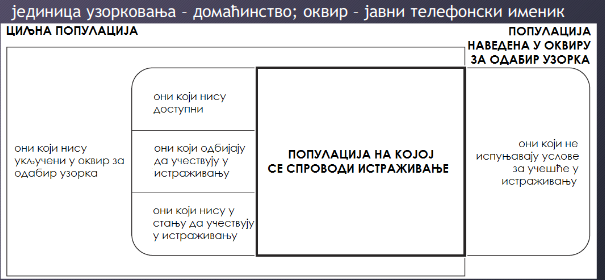
\includegraphics[scale=0.5]{primer1}
\\[0.2cm]
Zašto uzorkovanje?
\\
\textbf{Potpuno} ispitivanje populacije 
(proučavanje tzv. \textbf{cenzusa}) je, u 
mnogim  slučajevima, neracionalno ili čak principijelno nemoguće. 
Čak i onda kada postoji mogućnost potpunog ispitivanja populacije 
istraživač se obično opredeljuje za \textbf{delimično} ispitivanje (proučavanje 
uzorka) jer je (u odnosu na potpuno ispitivanje):

\begin{itemize}
	\item jeftinije 
	\item brže
	\item kontrola tačnosti prikuplenih podataka je jednostavnija
	 i lakša
\end{itemize}

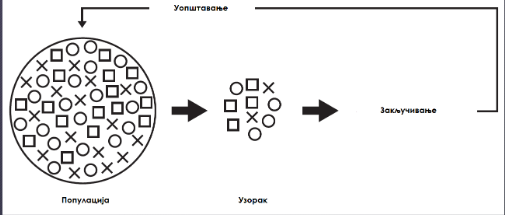
\includegraphics[scale=0.55]{primer2}
\\[0.25cm]

Termin populacija odnosi se na skup entiteta istovrsnih u odnosu 
na jedno ili više zajedničkih svojstava, koja se mogu posmatrati. 
Ipak, entiteti, iako \textbf{istovrsni}, \textbf{nisu istovetni}.
\\ 
Određivanje populacije 
predstavlja značajnu i, neretko, tešku fazu istraživanja. Populacija 
mora biti definisana: pojmovno (u smislu svog sadržaja - šta su 
entiteti, a šta jedinice uzorkovanja?), prostorno i vremenski.

\textbf{Obeležje} ('study variable') - posmatrana zajednička 
karakteristika 
svih entiteta u populaciji, tj. preciznije, izvesno varijabilno 
svojstvo od interesa, koje je određeno za svaki entitet u populaciji.
\footnote{Obeležje najčešće nije neko od definicionih svojstava
populacije.}

\subsection{Tipovi obeležja}

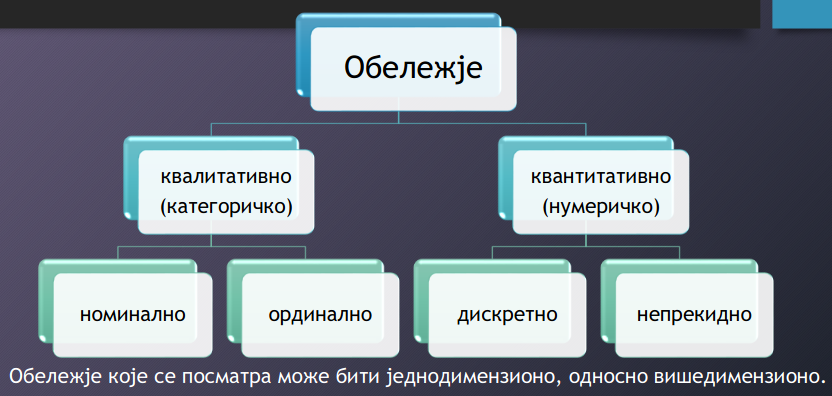
\includegraphics[scale=0.4]{primer3}
\pagebreak
\\
\underline{Primer}: tipovi obeležja
\begin{itemize}
	\item kvalitativna
	\begin{itemize}
		\item nominalna
			\begin{itemize}
				\item boja očiju, krvna grupa
				\item etnička / verska pripadnost 
				\item radna mesta na fakultetu
				\item raspoloženje građana Srbije prema pristupanju
				u EU
				\item posedovanje profila na društvenim mrežama
			\end{itemize}
		\item ordinalna
			\begin{itemize}
				\item nivo akademskih studija
				\item čin oficira u vojsci
				\item ocena restorana na Tripadvisor
				\item stanje pacijenta
				\item intezitet bola
			\end{itemize}
	\end{itemize}
	\item kvantitativna
	\begin{itemize}
		\item diskretna
			\begin{itemize}
				\item broj stanovnik sa pravom glasa u određenoj
				opštini
				\item broj blizanaca rođenih u toku godine u
				određenoj regiji
				\item broj kućnih ljubimaca u domaćinstvu
			\end{itemize}
		\item neprekidna
			\begin{itemize}
				\item visina, težina, starost, IQ
				\item dužina lista određene biljne vrste
				\item koncetracija soli u morskoj vodi
			\end{itemize}
	\end{itemize}
\end{itemize}

\underline{Primer}: populacija i obeležje
\begin{itemize}
\item 
\textcolor{red}{Populacija}: skup studenata koji su upisali Uvod u teoriju uzoraka školske 2019/20. godine.
\\
\textcolor{blue}{Obeležje}: pol; broj položenih ispita, broj položenih ESPB bodova,prosečna ocena svih položenih ispita –zaključno sa rokom Januar 2 ove školske godine; ocena na kursu Statistika
\item
\textcolor{red}{Populacija}: skup svih poljoprivrednih gazdinstava u Srbiji(referentni period–oktobar/novembar2018)
\\
\textcolor{blue}{Obeležje}:površina korišćenog poljoprivrednog zemljišta;
broj grla stoke; primenjeni proizvodni metodi

\item
\textcolor{red}{Populacija}: skup svih domaćinstava u regionu Šumadije i Istočne Srbije(referentni period –2017. g)
\\
\textcolor{blue}{Obeležje}: lična potrošnja domaćinstva (mesečni prosek)

\item
\textcolor{red}{Populacija}: jedna serija LED sijalica izvesnog proivođača.
\\
\textcolor{blue}{Obeležje}: dužina radnog veka sijalice u satima.


\item
\textcolor{red}{Populacija}: skup svih meseci u periodu od 2000. do 2016. g.
\\
\textcolor{blue}{Obeležje}: mesečni broj vetrovitih dana u Vršcu	
\end{itemize}


Obeležje se može shvatiti kao funkcija koja entitetima u populaciji 
pridružuje realne brojeve ili neke druge vrednosti.
\\
Neka je data 
populacija sa 𝑁 jedinica, koje su u okviru za odabiruzorka označene 
brojevima iz skupa $\omega={1,2,...,𝑁}$ (i time jednoznačno određene)i neka 
je 𝑌 obeležje od interesa.Neka je sa $y_k$ označena vrednost obeležja 
𝑌 entiteta označenog sa 𝑘. \\

Zadatak pri istraživanju obično se svodi na donošenje zaključaka o 
(nepoznatoj) vrednosti realne funkcije 
$$\theta=f(y_{1},y_{2},,y_{n})$$, koja se naziva 
\textbf{populacijska vrednost} ('population value') ili 
\textbf{parametar populacije}.
\\

Najčešće funkcije koje se pojavljuju kao parametri populacije:
\begin{itemize}
	\item Kvantitativna obeležja
		\begin{itemize}
			\item populacijska srednja vrednost ('population mean')
			$$m_Y  = m = \frac{1}{N}\sum_{k=1}^{N}y_{K}$$
			\item populacijski total ('population total')
			$$\tau_{Y} = \tau = \sum_{k=1}^{N}y_{K} = Nm_Y $$
			\item populacijska disperzija ('population variance')
			/ standardno odstupanje
			$$\sigma^2_Y = \sigma^2 = 
			\frac{1}{N-1}\sum_{k=1}^{N}(y_K - m_Y)^2$$ i
			$$\sigma_Y = \sigma = \sqrt{\sigma^2_Y}$$
		\end{itemize}
	\item Kvalitativna obeležja
		\begin{itemize}
			\item populacijska proporcija ('population proportion')
			\item populacijska medijana, kvantili, moda...
		\end{itemize}
\end{itemize}

Ideja je da se zaključci o populacijskim vrednostima donose na osnovu 
informacija dobijenih ispitivanjem uzorka.

„Dobar“ uzorak ima osobinu \textbf{reprezentativnosti}. To je uzorak 
koji predstavlja „umanjenu“, a nikako „iskrivljenu“, niti „uveličanu“ 
sliku jednog dela populacije. Uzorak sa ovom osobinom verno odslikava 
strukturu populacije koju predstavlja, „izgledajući“ kao i populacija 
u svim aspektima relevatnim za istraživanje.
\\
\pagebreak
\\
Na reprezentativnost uzorka utiču:
\begin{itemize}
	\item tip uzorka (prema metodu odabira)
	\item veličina uzorka
	\item varijabilnost posmatranog obeležja
\end{itemize}

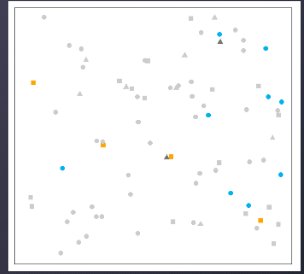
\includegraphics[scale=0.5]{primer4}

\textbf{Plan uzorkovanja} ('sampling design') poseduje dve osnovne 
komponente: 
	\begin{itemize}
		\item metod odabira uzorka
		\item metod zaključivanja
	\end{itemize}
\textbf{Metod odabira uzorka} je postupak kojim se biraju elementi
populacije u uzorak, uz određivanje adekvatnog obima uzorka.
\\
Ovi metodi se mogu podeliti u dve grupe:
	\begin{itemize}
		\item \textbf{Verovatnosno uzorkovanje} 
		('probability sampling')
		\item \textbf{Neverovatnosno uzorkovanje}
		('nonprobability sampling')
	\end{itemize}	
	
	
\subsection{Nevereovatnosno uzorkovanje}
Ovakvi metodi uzorkovanja ne zasnivaju se na teoriji verovatnoća, 
nego na određenim kriterijumima istraživača. 
\\
Dakle, njihova osnovna 
osobina jeste da se uzorkovanje vrši na osnovu 
\textbf{subjektivne procene 
istraživača}, a ne slučajnim izborom. Njima se pribegava onda kada je, 
zbog ograničenih vremenskih rokova, iznosa troškova i osetljivosti 
predmeta istraživanja (etičkih obzira), teško sprovesti slučajno 
uzorkovanje.

\begin{itemize}
	\item \textcolor{green}{Prednosti}:
	efikasnije se primenjuju kod eksplorativnih istraživanja (pilot 	
	istraživanja, studije u cilju dokazivanja koncepta, kvalitativna 
	istraživanja, studije za generisanje hipoteza), čiji cilj nije 
	precizno zaključivanje o parametrima populacije na osnovu 
	reprezentativnog uzorka.
	\item \textcolor{red}{Mane}:
	nije moguće određivanje kvaliteta uzorka, a samim tim ni 
	kvantifikovanje tačnosti zaključivanja (zaključivanje je ovde 
	analitičko).
\end{itemize}

\includegraphics[scale=0.5]{primer5}



\subsection{Verovatnosno uzorkovanje}
Ovakvi metodi uzorkovanja zasnivaju se na teoriji verovatnoća, tj. na 
„planiranoj“ slučajnosti. Mogući uzorci su faktički matematički 
konstruisani, i za svakog od njih poznata je verovatnoća da bude 
odabran. Dakle, uzorkovanje se vrši u skladu sa raspodelom 
verovatnoća, definisanom na kolekciji svih mogućih uzoraka.

\textbullet Neka je sa $\Omega $ označen skup oznaka jedinica u populaciji 
i neka $s \subset \Omega $
predstavlja uzorak.
Verovatnosno uzorkovanje se zasniva na poznavanju raspodele verovatnoća $p(\bullet)$:
$$ p(s) \geq 0,	 \forall s \subset \Omega,
 \sum_{s \subset \Omega} p(s) = 1 $$

Slučajan uzorak $S$ je onda slučajan skup oznaka jedinica sa 
raspodelom verovatnoća:
$$P\{S=s\} = p(s), \forall s \subset \Omega$$

\includegraphics[scale=0.5]{primer6}

\textcolor{green}{Prednosti}:
\begin{itemize}
 
	\item doslednom primenom isključuje se postojanje bilo kakve 
	pristrasnosti, 
	što doprinosi postizanju objektivnosti istraživanja
	\item viši nivo pouzdanosti rezultata istraživanja
	\item mogućnost procene / kvantifikovanja uzoračke greške
	\item povećane su šanse za donošenje valjanih zaključaka o 
	čitavoj populaciji, uopštavanjem rezultata dobijenih ispitivanjem uzorka

\end{itemize}
\textcolor{red}{Mane}:
\begin{itemize}
	\item 
	uglavnom se tiču potreba za vremenom, resursima, finansijama i 
	ljudstvom (npr. potrebno je posedovati kompletan okvir za odabir 
	uzorka)

\end{itemize}
\subsection{Osnovni pojmovi, nastavak}
Ako se na slučajan način (sa unapred određenom verovatnoćom) odabere 
jedna jedinica iz populacije, vrednost obeležja koju ona ima nije 
unapred poznata / određena. To znači da se vrednost obeležja slučajno 
odabrane jedinice može shvatiti kao realizacija slučajne veličine. 
Raspodela verovatnoća te slučajne veličina naziva se 
\textbf{raspodela 
obeležja}\footnote{Zadatak matematičke statistike je određivanje
raspodele obeležja ili određivanje bar nekih opštih numeričkih 
karakteristika te raspodele}.
\\[0.2cm]
\textbf{Statistika} ('statistic') je funkcija vrednosti obeležja registrovanih 
na jedinicama iz odabranog uzorka, u kojoj eventualno mogu figurisati 
i neke poznate konstante.\footnote{Statistika je slučajna veličina sa svojom raspodelom verovatnoća, koja se naziva \textbf{uzoračka raspodela}}
\\


Statistike su značajne jer se često koriste za formiranje 
\textbf{ocena} ('estimator') parametara populacije. Realizovane vrednosti statistika su realni brojevi koji tada daju \textbf{ocene} 
('estimate') nepoznatih parametara.
Npr. ako je  $\theta$ nepoznata populacijska vrednost onda je 
$\hat{\theta} = \hat{\theta(s)}$ statistika, koja predstavlja \textbf{tačkastu ocenu} ('point 
estimator') parametra. 

Često korišćene statistike ($n(S)$ predstavlja obim uzorka $S$):
\begin{itemize}
\item uzoračka srednja vrednost
	$$ \overline{Y} = \frac{1}{n(S)} \sum_{k \in S}y_k$$
\item uzorački total
	$$ T = n(S)\overline{Y}$$
\item uzoračka disperzija / standardno odstupanje 
	$$ \overline{S}^2 = \frac{1}{n(S) - 1}\sum_{k \in S}(y_k - \overline{Y})^2, \overline{S} = \sqrt{\overline{S}^2}$$
\item uzoračka proporcija 
\item uzoračka medijana, kvantili, moda
\end{itemize}
Neka je $\hat{\theta}$ tačkasta ocenapopulacijske vrednosti
$\theta$. Ona je:
\begin{itemize}
\item \textbf{nepristrasna} ('unbiased')
\\
ako jednakost \textbf{$E\hat{\theta} = \theta$} važi za svaku 
vrednost 
parametra $\theta$; ako ocena $\hat{\theta}$ nije nepristrasna onda 
se ona naziva \textbf{pristrasna ocena}, a vrednošću razlike  
$B(\hat{\theta}) := E\hat{\theta} - \theta$ meri se njena 
\textbf{pristrasnost}.
\item \textbf{precizna} ('precise')
\\
ako je disperzija $D\hat{\theta} = E(\hat{\theta} - E\hat{\theta})^2$
ocene $\hat{\theta}$ mala (teži 0).

\item \textbf{tačna} ('accurate')
\\
ako je srednje kvadratna greška 
$MSE(\hat{\theta}) := E(\hat{\theta}-\theta)$ ocene $\hat{\theta}$ 
mala.\footnote{važi i jednakost: 
$MSE(\hat{\theta}) = D\hat{\theta} + (B(\hat{\theta}))^2$, pa je 
ocena tačna ako je i precizna i nepristrasna.}

\end{itemize}
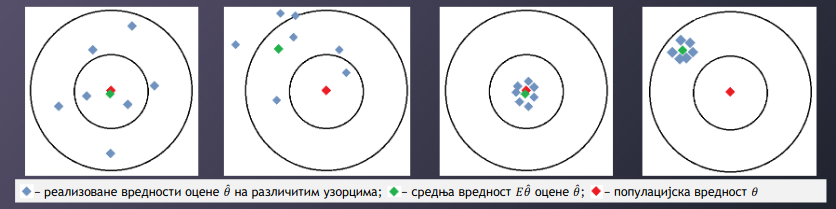
\includegraphics[scale=0.5]{primer7}


\section{nedelja}
\subsection{(Prost) slučajan uzorak}
Kod (prostog) slučajnog uzorkovanja ('simple random sampling')
\textbf{jedinica posmatranja = jedinica uzorkovanja}.
\\
Neka je data populacija sa $N$ jedinica, koje su u okviru za 
odabir uzorka označene brojevima iz skupa $\Omega = \{1, 2, ..., N\}$ i neka je 
$Y$ obeležje od interesa. Bira se uzorak obima $n$.
\\

Može biti:
\begin{itemize}
	\item bez ponavljanja (SRSWOR)
	\item sa ponavljanjem (SRSWR)
\end{itemize}


\subsection{SRSWOR}
Predstavlja jedan od najjednostavnijih i najstarijih metoda odabira 
uzorka.
Raspodela verovatnoća $p(\cdot)$ na kolekciji svih uzoraka $s \subset 
\Omega$ data je sa:

\begin{equation}
p(s) = \begin{cases}
	\binom{N}{n}^{-1}, \text{ako je obim uzorka } s \text{ jednak } n 
	\\[0.2cm]
	\ 0, \text{ inače} 
\end{cases}
\end{equation}


Dakle, ovde se svaki od $\binom{N}{n}$ mogućih podskupova skupa 
 $\Omega$ kardinalnosti $n$ sa 
podjednakom (pozitivnom) verovatnoćom može odabrati kao uzorak


Pomenuti plan obično se u praksi implementira jednim od sledeća dva 
ekvivalentna postupka:
\begin{itemize}
	\item odabir uzorka vrši se kroz 𝑛izvlačenja („koraka“) na 
	slučajan način, pri čemu je u svakom koraku verovatnoća 
	izvlačenja bilo koje od jedinica, koje u ranijim koracima nisu 
	odabrane u uzorak, ista
	\item odabir uzorka vrši se kroz niz \textbf{nezavisnih}
	izvlačenja na 
	slučajan način \textbf{iz cele populacije}, pri čemu je u svakom 
	koraku 
	verovatnoća izvlačenja bilo koje od 
	jedinica ista $\binom{1}{N}$,uz 
	odbacivanje jedinica ranije odabranih u uzorak i ponavljanje 
	koraka sve dok se ne dobije uzorak obima 𝑛
\end{itemize}

Uzorak odabran na opisani način može se prikazati i 
kao \textbf{uređen} niz $j_1, j_2,..., j_n$oznaka jedinica koje su se našle u 
uzorku($j_k$je oznaka $k$-te jedinice zadržane u uzorku)
\\

Uzorak odabran na opisani način može se prikazati i kao uređen niz 
$j_1,j_2,...,j_n$ oznaka jedinica koje su se našle u uzorku
($j_k$ je oznaka $k$-te) 
jedinice zadržane u uzorku).Pod uzorkom se, takođe, podrazumeva i 
pripadni niz $y_{j1},y_{j2},...,y_{jn}$vrednosti posmatranog obeležja 
$Y$ registrovanih na odabranim jedinicama.
\\

Parovi $(j_k,y_{jk}), k=\overline{1,𝑛}$, predstavljaju 
\textbf{podatke dobijene u 
istraživanju}.

\subsection{SRSWR}
\textbullet	Odabir uzorka vrši se kroz $N$ nezavisnih izvlačenja na 
slučajan način, i to uvek iz kompletne populacije, pri čemu je u 
svakom koraku verovatnoća izvlačenja bilo koje od jedinica ista i 
jednaka $\frac{1}{N}$.
\\
\textbullet 
Raspodela verovatnoća $p(\cdot)$ na kolekciji svih uzoraka
$s \in \Omega^n$kao 
uređenih 
nizova dužine 𝑛sa dozvoljenim ponavljanjem elemenata data je sa
$p(s) = N^{-n}$

\subsection{Izvlačenje jedinice na slučajan način}
Slučajan odabir jedinice (iz populacije u uzorak) vrši se korišćenjem 
\textbf{slučajnih} i \textbf{pseudoslučajnih brojeva}.
\\
Slučajni brojevi obično se dobijaju pomoću tzv. 
\textbf{fizičkih
generatora}
(TRNG –'true random number generator').
\begin{itemize}
\item u makro svetu: bacanje fer novčića / 
kockica, slučajan izbor karte iz špila / kuglice 
iz kutije, rulet itd.
\item u mikro svetu: prirodni fenomeni za koje važe zakonitosti kvantne mehanike, šum itd.
\end{itemize}
Oni su sadržani u tzv. \textbf{tablicama slučajnih brojeva}.
\\[0.1cm]
Pseudoslučajni brojevi se dobijaju pomoću tzv. \textbf{programskih generatora}
(PRNG –'pseudorandom number generator').
To su računarski programi koji koriste izvestan algoritam za dobijanje niza brojeva čija 
svojstva, u određenoj meri, oponašaju svojstva niza slučajnih brojeva.

\subsection{Novi pojmovi}
\begin{itemize}
	\item \textbf{Indikator uključenja} ('inclusion indicator')
	\begin{equation}
		I_k = \begin{cases}
		1, \text{  ako je jedinica označena sa } k \text{ odabrana u uzorak} \\
		0, \text{  inače}
		\end{cases}
	\end{equation}
	\item \textbf{Verovatnoća uključenja} ('inclusion probability') 
	prvog, odnosno drugog reda:\\
	$\pi_k$ - verovatnoća da jedinica označena sa $k$ bude odabrana u uzorak\\
	$\pi_{kl}$ - verovatnoća da i jedinica označena sa $k$ i jedinica označena sa $l$ budu 
	odabrane u uzorak
	\item \textbf{'Težina' uzorkovanja} ('sampling weight')
	recipročna vrednost očekivanog broja pojavljivanja jedinice označene sa $k$ u uzorku
	(što 
	se, kod uzorka bez ponavljanja, svodi na recipročnu vrednost verovatnoće uključenja 
	prvog reda $\pi_k$) \footnote{može se interpretirati kao broj jedinica u populaciji 
	koje reprezentuje jedinica označena sa $k$}.
	
\end{itemize}
\subsection{SRSWOR VS SRSWR}
\begin{center}
\begin{tabular}{|p{6cm}|p{6cm}|}
\hline
SRSWOR & SRSWR \\
\hline
Verovatnoća uključenja prvog reda: 
&
Verovatnoća uključenja prvog reda: \\
$ \pi_k = \frac{n}{N} \text{ za svako } k$
&
$ \pi_k = 1 - (\frac{N-1}{N})^n \text{ za svako } k $
\\
\hline

Verovatnoća da će jedinica označena sa $k$ biti odabrana u uzorak u $j$-tom koraku:
&
Verovatnoća da će jedinica označena sa $k$ biti 
odabrana u uzorak u $j$-tom koraku:
\\

$\frac{1}{N}$
&
$\frac{1}{N}$\\
\hline

&
Verovatnoća da će jedinica označena sa $k$ biti odabrana u uzorak više od jedanput:\\

&
$1 - \big(\frac{N-1}{N}\big)^{n-1}\big(\frac{N-1-n}{N}\big)$ \\
\hline

Očekivanibroj pojavljivanja jedinice označene sa $k$ u uzorku:
&
Očekivanibroj pojavljivanja jedinice označene sa $k$ u uzorku: \\
$\pi_k$
&
$\frac{n}{N}$ \\
\hline
Verovatnoća uključenja drugog reda:
&
Verovatnoća uključenja drugog reda: \\

$\pi_{kl} = \frac{n(n-1)}{N(N-1)} \text{ za } k \neq l$
&
$\pi_{kl} = 1 - 2\big(\frac{N-1}{N}\big)^n 
+ \big(\frac{N-2}{N}\big)^n \text{ za } k \neq l$\\
\hline

\end{tabular}
\end{center}



\subsection{Pristupi prilikom zaključivanja}

\begin{center}
\begin{tabular}{|c|c|}
\hline
\makecell{\textbf{pristup zasnovan na metodu odabira uzorka}
 \\ 
 \textbf{('design-based approach')}}
&
\makecell{\textbf{pristup zasnovan na modelu}
\\ \textbf{('model-based approach')}
}

\\
%$$P\{\hat{\theta} = m\} = \sum_{s:\hat{\theta}(s)=m}p(s)$$
\hline
\makecell {
	uzoračka raspodela statistike je\\
	\textbf{diskretna raspodela verovatnoća}:\\
	ako je $\hat{\theta} = \hat{\theta}(S)$ statistika, onda važi: \\
	$P\{\hat{\theta} = m\}=\sum_{s:\hat{\theta}(s)=m}p(s)$\\
	a njeno matematičko očekivanje i disperzija \\ 
	izračunavaju se po formulama:\\
	$E\hat{\theta} = \sum_{m}mP\{\hat{\theta} = m\}
	= \sum_{s}\hat{\theta}(s)p(s)$ \\
	$D\hat{\theta} = \sum_{s}(\hat{\theta}(s) - E\hat{\theta})^2 p(s)$
}
&
\makecell {
 uzoračka raspodela statistike\\
 je \textbf{neka} jednodimenziona\\ 
 \textbf{raspodela verovatnoća} određena \\
 zajedničkom raspodelom verovatnoća\\
 pretpostavljenog modela populacije
}
\\
\hline
\makecell {
	\textbf{nepristrasnost} tačkaste ocene\\
	$E\hat{\theta}$ \textbf{u odnosu na metod odabira uzorka}
}
&
\makecell {
	\textbf{nepristrasnost} tačkaste ocene\\
	$E\hat{\theta}$ \textbf{u odnosu na metod model}
}\\
\hline

\end{tabular}
\end{center}


\subsection{SRSWOR VS SRSWR tačkaste ocene}
\begin{center}
\begin{tabular}{|c|c|c|c|}
\hline
&
\makecell {
	SRSWOR
}
&
\makecell {
	SRSWR
}
&
\makecell {
	SRSWR\\
	(u obzir se uzimaju samo različite jedinice)
}\\
\hline


\makecell {
	tačkasta ocena $\hat{m}_Y$
}
&
\makecell {
	$\frac{1}{n} \sum_{k \in S}y_k$
}
&
\makecell {
	$\frac{1}{n} \sum_{k=1}^{n}y_{jk}$
}
&
\makecell {
	$\frac{1}{n_D} \sum_{k}y_{(k)}$ 
}\\
\hline


\makecell {
	$E\hat{m}_Y$
}
&
\makecell {
	$m_Y$
}
&
\makecell {
	$m_Y$
}
&
\makecell {
	$m_Y$
}\\
\hline


\makecell {
	$D\hat{m}_Y$
}
&
\makecell {
	$\frac{\sigma^2}{n}\big(1 - \frac{n}{N}\big)$
}
&
\makecell {
	$\frac{N-1}{N} \frac{\sigma^2}{n}$
}
&
\makecell {
	$\sum_{k=1}^{N-1}\frac{k^{n-1}}{N^n}\sigma^2$
}\\
\hline



\makecell {
	tačkasta ocena $D\hat{m}_Y$
}
&
\makecell {
	$\frac{\overline{S}^2}{n}\big(1 - \frac{n}{N}\big)$
}
&
\makecell {
	$\frac{\overline{S}^2}{n}$
}
&
\\
\hline


\end{tabular}
\end{center}
\footnote{$n_D$ je \textbf{efektivan obim uzorka}, tj. obim redukovanog
	uzorka $(y_{(1)}, y_{(2)}, ..., y_{n_D})$ u kome su izostavljena
	eventualna ponavljanja jedinica iz originalnog uzorka
}


gde je $\sigma^2$ (nepoznata) populacijska disperzija, a $\overline{S}^2$
(poznata) uzoračka disperzija. 
\footnote{može se pokazati da je $\hat{S}^2$ nepristrasna ocena $\sigma^2$}


\subsection{Novi pojmovi}


\end{document}